% !TeX root = ../main.tex

\section{Introduction}
\label{sec:introduction}

% 总结全文，为什么要SAR时序监测

Balsa (\textit{Ochroma pyramidale}) is a fast-growing tropical tree species whose wood combines low density with useful mechanical properties, making it valuable for lightweight structures, including wind-turbine blade cores~\citep{Borrega2015Balsa_mechanics,Midgley2010Balsa}. Ecuador is a major source of commercial balsa, and its plantations can undergo management-related turnover on cycles of only a few years under productive tropical conditions~\citep{GonzalezOsorio2010Balsa,CanadasLopez2019BalsaGrowth}. Reconstructing these short-rotation dynamics therefore requires a long and temporally continuous observation record spanning multiple disturbance events within the same stand, rather than a single disturbance label~\citep{Du2022GlobalPlantingYears,Li2022EucalyptusHistory}. This requirement is difficult to meet with optical satellite imagery because persistent cloud cover in tropical Ecuador disrupts temporal continuity and can leave critical disturbance periods unobserved~\citep{DelgadoAguilar2017EcuadorSAR}. Sentinel-1 synthetic aperture radar (SAR) provides a cloud-independent, long-term observation record with frequent repeat acquisitions~\citep{Torres2012S1}, providing the observational basis to investigate whether recurrent stand disturbances can be reliably resolved from long-term SAR trajectories.

% SAR监测的难点

Even with dense SAR observations, reconstructing recurrent stand disturbances remains challenging. Sentinel-1 backscatter responds not only to canopy structure but also to moisture conditions, surface roughness, phenological state, and acquisition geometry, introducing temporal variability that can overlap the signal of structural change~\citep{Reiche2018Bayesian,Doblas2020harmonic,Matthew2021BFAST,vanDerWoude2024S1Disturbance,BorlafMena2023Seasonality}. Seasonality and viewing geometry can alter forest backscatter even in the absence of management change, while the sensitivity of C-band SAR to a given surface-state transition also varies with land-surface conditions~\citep{BorlafMena2023Seasonality,Zhao2021SARExclusion}. Consequently, absolute backscatter does not uniquely identify plantation state across stands and environments. As a stand changes after disturbance and recovery, a fixed historical reference may also cease to represent its current condition~\citep{Li2022EucalyptusHistory,Ygorra2023ReCuSum}. A temporally adaptive reference is therefore central to recurrent disturbance monitoring, allowing persistent structural departures to be distinguished from normal SAR variability.

% literature review

Optical and SAR-based time-series studies have addressed different aspects of forest and plantation change monitoring. Multi-decadal Landsat records have been used to identify successive plantation rotations and quantify productivity~\citep{McMahon2019EucalyptusRotations}, while other optical time-series approaches have reconstructed planting history, harvest timing, generation, rotation length, and stand age in short-rotation plantations~\citep{Du2022GlobalPlantingYears,Li2022EucalyptusHistory}. More recently, month-resolved Landsat--Sentinel observations have improved harvest-date localization and stand-age estimation~\citep{Huang2026EucalyptusAge}. Sentinel-1 studies, in contrast, have focused mainly on disturbance detection and near-real-time monitoring, including Bayesian monitoring, continuous change detection, cumulative sum (CUSUM)-based methods, and coherence-based approaches~\citep{Reiche2018Bayesian,Bullock2022CCDC_S1,RuizRamos2020CUSUMSMC,Ygorra2021CuSum,Akbari2022ClearCut}. Sensitivity to management-related and low-intensity forest disturbances has also been demonstrated~\citep{vanDerWoude2024S1Disturbance,Aquino2022LowIntensity}. Yet reconstructing multiple dated disturbances within the same managed stand from a near-decadal SAR record remains largely unexplored.

% 引出CUSUM方法: 已有 SAR 能检测变化, CUSUM 能积累持续偏离,
% ReCuSum 能处理多变化, CuSum NRT 已经使用滑窗,
% 但仍缺少面向长期林分 recurrent history 的 local-reference 设计

CUSUM methods provide an interpretable way to accumulate persistent departures from a temporal reference~\citep{Page1954CUSUM}. They have been used for continuous forest monitoring and tropical disturbance detection~\citep{RuizRamos2020CUSUMSMC,Ygorra2021CuSum}. ReCuSum extends this principle to multiple disturbances through recursive segmentation~\citep{Ygorra2023ReCuSum}, whereas CuSum NRT applies CUSUM iteratively to short sliding time series to reduce detection delay~\citep{Ygorra2024CuSumNRT}. The remaining challenge in short-rotation plantations is to repeatedly renew the local reference without making later detections contingent on earlier segmentation, while retaining sufficient temporal context to reconstruct a consistent stand-level disturbance history.

% 总结，引出研究内容

We therefore propose \textit{Windowed CUSUM}, which repeatedly renews local references through overlapping temporal windows and retains only negative, statistically supported candidates within each window's central decision interval before consolidating them into recurrent stand-disturbance histories (Fig.~\ref{fig:workflow}). This study aims to (1) characterize the within-stand Sentinel-1 response to historical balsa disturbances; (2) evaluate whether Windowed CUSUM improves recurrent-event detection relative to alternative detectors and remains robust to stand representation, polarization, temporal configuration, and statistical assumptions; and (3) reconstruct recurrent plantation disturbance histories and characterize their spatial and temporal dynamics using stand-level event counts and inter-disturbance intervals.

\begin{figure*}[pos=!htbp]
    \centering
    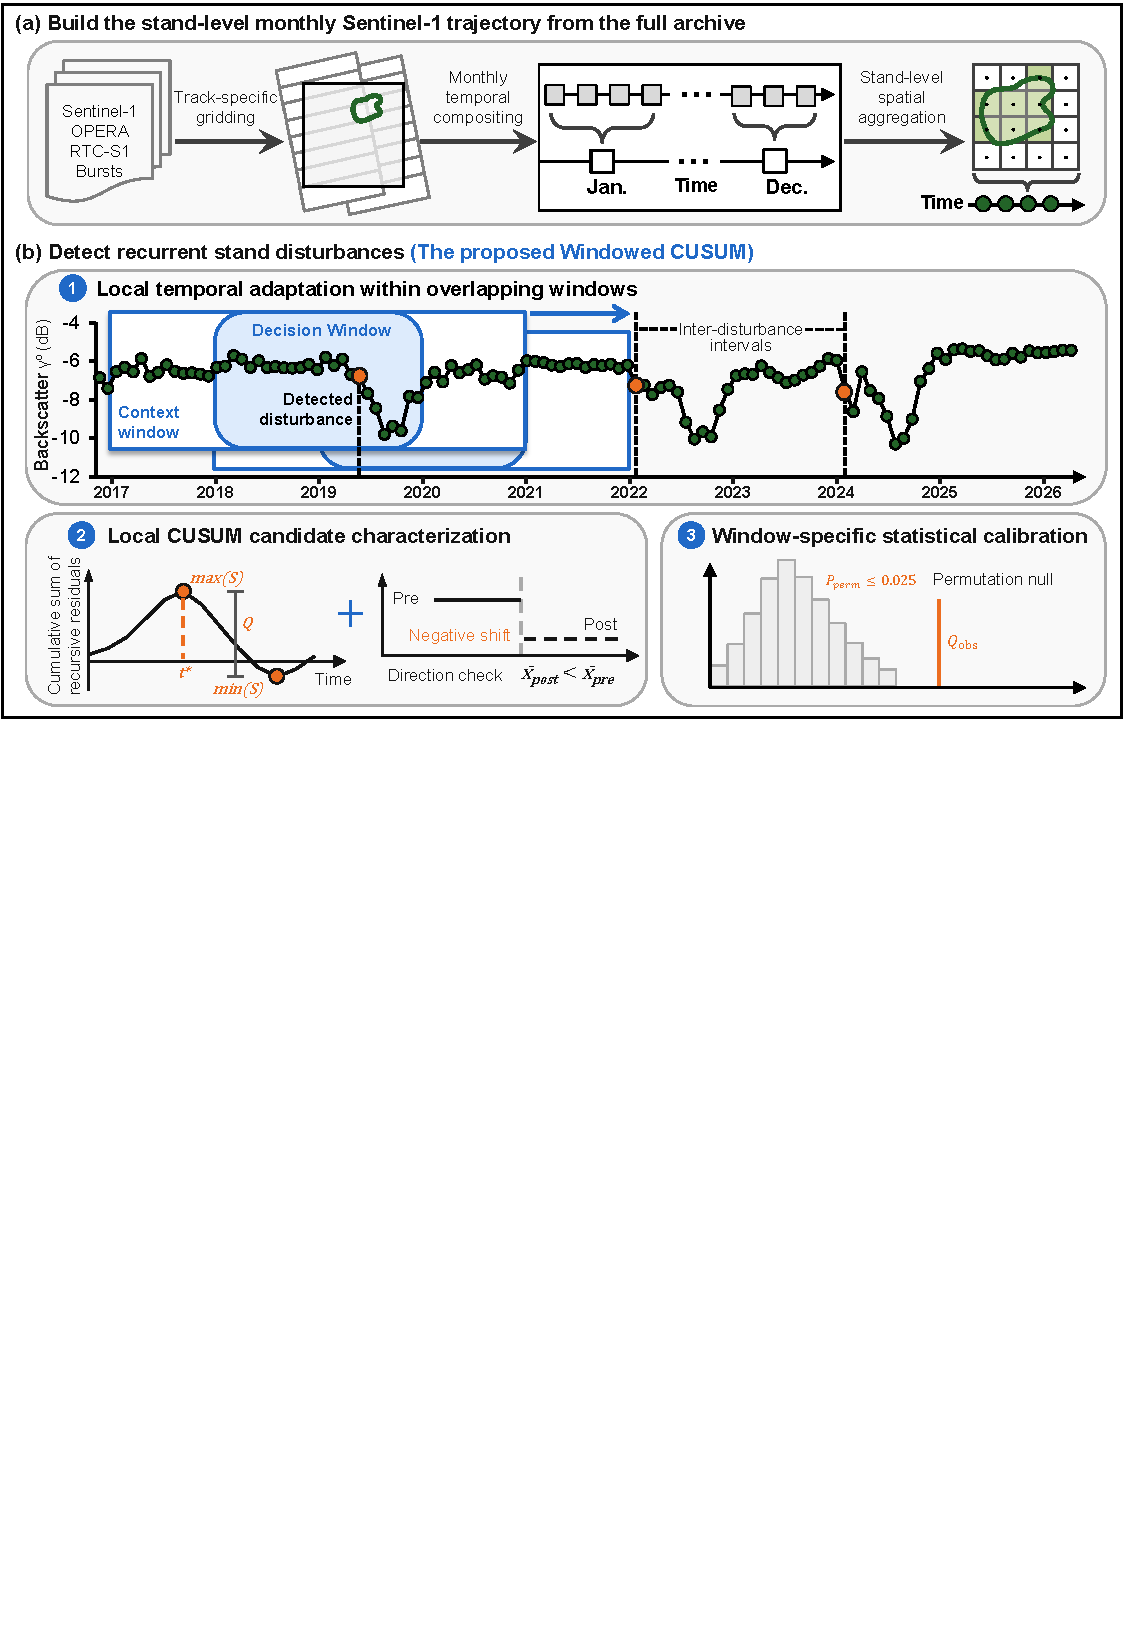
\includegraphics[width=\linewidth]{figures/fig03_workflow.pdf}
    \caption{Conceptual illustration of Windowed CUSUM for one observed balsa stand. (a) Construction of track-specific monthly stand-level Sentinel-1 trajectories. (b) Localization, screening, and consolidation of recurrent disturbance candidates. Within each window, CUSUM identifies candidate magnitude and timing, negative departures are screened against a window-specific permutation null, and accepted candidates are consolidated across overlapping windows.}
    \label{fig:workflow}
\end{figure*}


